\documentclass[t]{beamer}

% --- Theme and Color Setup ---
\usetheme{Madrid}

% Define the custom Orange color
\definecolor{MyOrange}{RGB}{230, 85, 10} 

% Apply the orange color to the structure
\usecolortheme[named=MyOrange]{structure}

% Fix footer colors to match the orange theme
\setbeamercolor{palette primary}{bg=MyOrange,fg=white}
\setbeamercolor{palette secondary}{bg=MyOrange!80!black,fg=white}
\setbeamercolor{palette tertiary}{bg=MyOrange!60!black,fg=white}
\setbeamerfont{caption}{size=\footnotesize}

% Packages
\usepackage[utf8]{inputenc}
\usepackage{hyperref}
\usepackage{tikz} 
\usepackage{booktabs}
\usepackage{natbib}
\usepackage{multicol}
\usepackage{xcolor}
\usepackage{amssymb}
\usepackage{tikz}
\usepackage{array}
\usetikzlibrary{arrows.meta, positioning, shapes}
\usepackage{tkz-euclide}
\usetikzlibrary{through}  
\usepackage[skins]{tcolorbox}



% Macros / notations
\newcommand\Q{\mathbb{Q}}
\newcommand\D{\mathbb{D}}
\newcommand\Z{\mathbb{Z}}
\newcommand\N{\mathbb{N}}
\newcommand\R{\mathbb{R}}
\newcommand\esp[1]{\mathbb{E}[{#1}]}
\newcommand{\probacond}[2]{%
\mathbb{P}(#1 \mid #2)%
}

\newcommand{\tikzAngleOfLine}{\tikz@AngleOfLine}
\def\tikz@AngleOfLine(#1)(#2)#3{%
\pgfmathanglebetweenpoints{%
\pgfpointanchor{#1}{center}}{%
\pgfpointanchor{#2}{center}}
\pgfmathsetmacro{#3}{\pgfmathresult}%
} 

\def\roundloop[#1]#2#3{%
\coordinate (rla) at (#2.east); 
\path   (#2)--++(#1) coordinate (rlb);
\tkzTgtFromP(#2,rla)(rlb)            
\node (rlb) at (rlb) [circle through={(tkzFirstPointResult)}] {};
\coordinate  (rlc) at (intersection 2 of #2 and rlb);
\coordinate  (rld) at (intersection 1 of #2 and rlb);         
\tikzAngleOfLine(rlb)(rld){\AngleStart}
\tikzAngleOfLine(rlb)(rlc){\AngleEnd} 
\tikzAngleOfLine(#2)(rlb){\AngleLabel}
\ifdim\AngleStart pt<\AngleEnd pt
\draw[thick,->]%
let \p1 = ($ (rlb) - (rld) $), \n2 = {veclen(\x1,\y1)}
in   
(rlb) ++(\AngleLabel:\n2) node[fill=white]{#3}
(rld) arc (\AngleStart:\AngleEnd:\n2); 
\else 
\draw[thick,->]%
let \p1 = ($ (rlb) - (rld) $), \n2 = {veclen(\x1,\y1)}
in   
(rlb) ++(\AngleLabel:\n2) node[fill=white]{#3}
(rld) arc (\AngleStart-360:\AngleEnd:\n2); 
\fi 
}


\def\pdftex@driver{pdftex.def}
\ifx\Gin@driver\pdftex@driver
  \def\pgfsys@color@unstacked#1{%
    \pdfliteral{\csname\string\color@#1\endcsname}%
  }
\fi


% --- Info ---
\title[Title]{Répétitions dans la génération de texte à partir de N-grams} % 
\subtitle{TIPE} % 
\author{Anonymous} % 



\begin{document}

% --- Slide 1: Title Page ---
\begin{frame}
    \titlepage
\end{frame}

% --- Motivation ---
\begin{frame}{Motivation} % 
    \begin{center}
        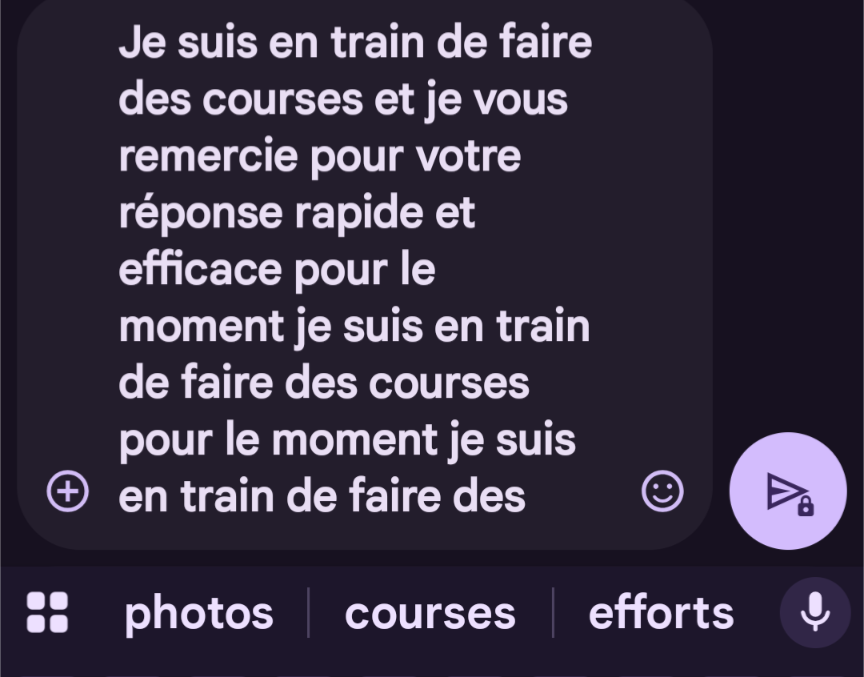
\includegraphics[scale=0.25]{images/predicteur_orthographique.png}
    \end{center}
\end{frame}


% --- Plan ---
\begin{frame}[c]{Plan} % 
    \begin{itemize}[<+->]
        \item Introduction
        \item L'algorithme BPE
        \item Génération de texte "greedy" (déterministe) % Existence de cycle, théorème de temps d'arrêt et comparaison avec les données
        \item Génération de texte stochastique (aléatoire) % Théorème d'existence de boucle et comparaison avec les données
        \item Conclusion % les "pseudo boucles" où le LLM raconte la même chose en boucle de différentes manières, comment on traite ce cas ? 
        % Optimisation des modèles à paramètres (interpolation, smoothing) sur la perplexity ET sur le temps de première répétition
        % Corrélation entre perplexity et temps de première répétition ?
    \end{itemize}
\end{frame}



\begin{frame}{Introduction : modèle N-gram}
    \begin{center}
        
\includegraphics[scale=0.2]{images/Ngram visuel.png}
    \end{center}
    \pause
    Hypothèse du modèle N-gram : \\
    \pause 
    $\forall n \geq N-1,$
    \begin{align*}
        &{\color{white}= } \probacond{X_{n+1}=x_{n+1}}{X_1 = x_1, X_2 = x_2, ..., X_{n}=x_{n}} \\
        &= \probacond{X_{n+1}=x_{n+1}}{X_{n -(N-1) +1} = x_{n -(N-1) +1}, ..., X_{n}=x_{n}}
    \end{align*} 
    \pause
    $(X_n)_{n \geq N}$ chaîne de Markov d'ordre N-1.
    %-> Chaînes de Markov d'ordre N-1
\end{frame}

\begin{frame}{Introduction : créer un modèle N-gram} % 
    \begin{center}
        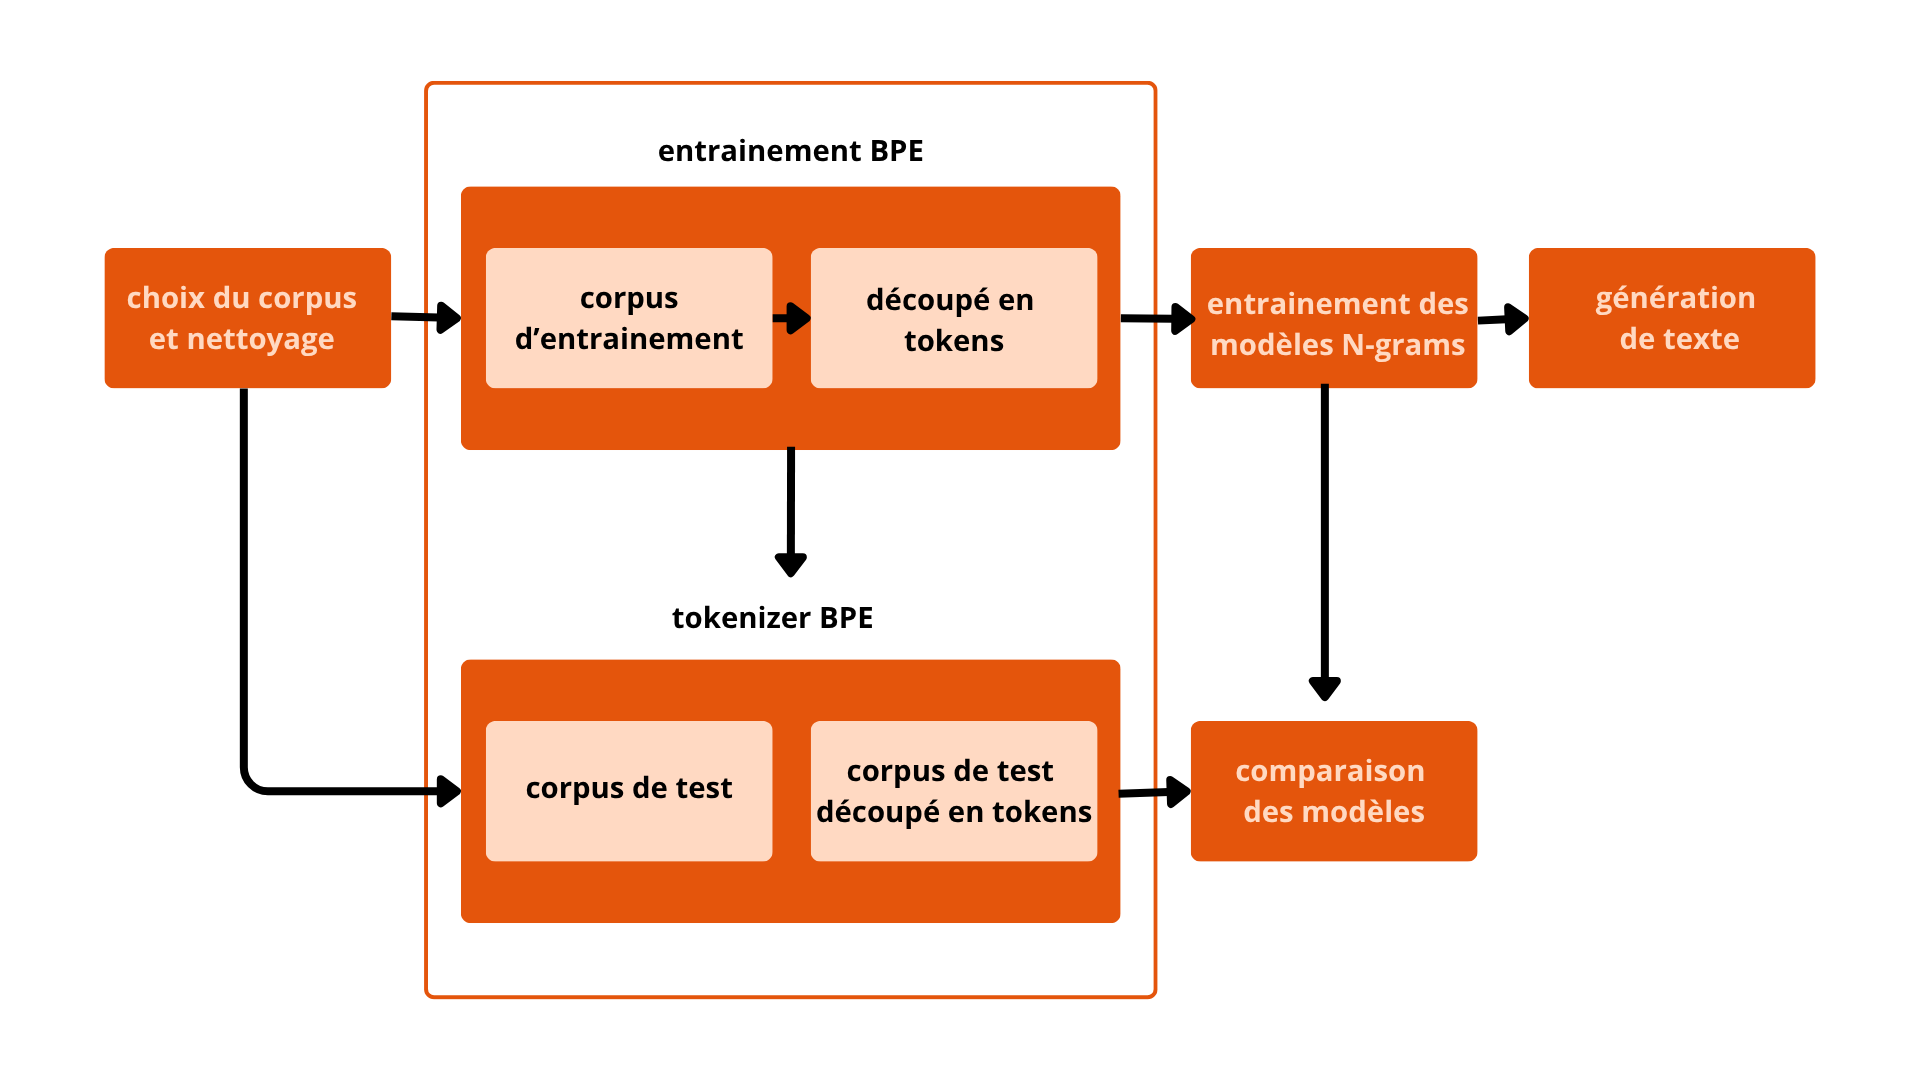
\includegraphics[scale=0.25]{images/choix du corpus et nettoyage.png}
    \end{center}
\end{frame}

% --- L'algorithme BPE ---
\begin{frame}[c]
    \centering
    \Huge \textcolor{MyOrange}{L'algorithme BPE} % 
\end{frame}

\begin{frame}{L'algorithme BPE : unité de morcellement du corpus} % 
    \begin{center} 
        \begin{tabular}{c|c|c|}
        Unité & Corpus d'entrainement & Corpus de test \\
        \hline
        & Il part, restez là. & Partez. \\[4ex]
        \pause
        {\color{red}Mot} & {\setlength{\fboxsep}{0.5pt} \colorbox{blue!20}{Il}%
\colorbox{yellow!60}{\_part}%
\colorbox{cyan!50}{,}%
\colorbox{red!50}{\_restez}%
\colorbox{green!60}{\_là}%
\colorbox{violet!60}{.}} & {\setlength{\fboxsep}{0.5pt} \colorbox{orange!60}{Partez}%
\colorbox{violet!60}{.}} \\[4ex]
        \pause
        {\color{red}Caractère} & I l \_ p a r t ,
        \_ r e s t e z \_ l à . & P a r t e z . \\[4ex]
        \pause
        {\color{red}Morphème} & {\setlength{\fboxsep}{0.5pt} \colorbox{blue!20}{Il}%
\colorbox{yellow!60}{\_part}%
\colorbox{cyan!50}{,}%
\colorbox{red!50}{\_rest}%
\colorbox{green!60}{ez}%
\colorbox{violet!60}{\_là}%
\colorbox{orange!60}{.}} & {\setlength{\fboxsep}{0.5pt} \colorbox{yellow!60}{Part}%
\colorbox{green!60}{ez}%
\colorbox{orange!60}{.}} \\
        \end{tabular}
    \end{center}
\end{frame}

\begin{frame}{L'algorithme BPE : l'idée} % 
    \begin{figure}[center]
        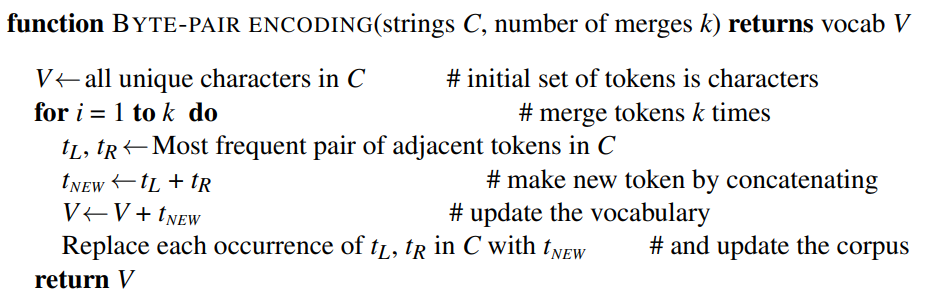
\includegraphics[width=9cm]{images/BPE_pseudo_code.png}
        \\ {\tiny Source : [1], adapté de Bostrom et Durett (2020)}
    \end{figure}
    \begin{figure}[center]
        \centering
        \text{Exemple d'apprentissage BPE}\par\medskip
        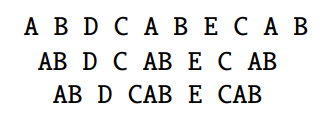
\includegraphics[width=6cm]{images/exemple BPE.png}
        \\ {\tiny Source : [1]}
    \end{figure}
\end{frame}


% --- Génération de texte "greedy" (déterministe) ---
\begin{frame}[c]
    \centering
    \Huge \textcolor{MyOrange}{Génération de texte "greedy" (déterministe)} % 
\end{frame}

\begin{frame}{Génération de texte "greedy" : existence d'une boucle} % 
    \pause 
    \begin{center}
        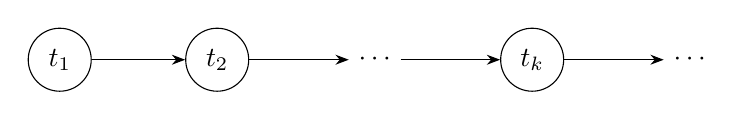
\begin{tikzpicture}[
            >=Stealth,
            vertex/.style={circle, draw, minimum size=8mm}
        ]

        % Sommets de la chaîne
        \node[vertex] (v1) at (0,0) {$t_1$};
        \node[vertex] (v2) at (2,0) {$t_2$};
        \node[] (v3) at (4,0) {$\cdots$};
        \node[vertex] (v4) at (6,0) {$t_k$};
        \node[] (v5) at (8,0) {$\cdots$};

        % Arêtes orientées
        \draw[->] (v1) -- (v2);
        \draw[->] (v2) -- (v3);
        \draw[->] (v3) -- (v4);
        \draw[->] (v4) -- (v5);


        \end{tikzpicture}
    \end{center}
    \pause 
    $\space$ \\ $\space$ \\
    \begin{center}
        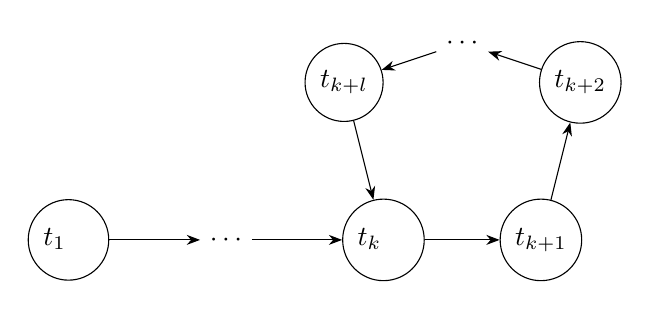
\begin{tikzpicture}[
            >=Stealth,
            vertex/.style={circle, draw, minimum size=8mm}
        ]

        % Sommets de la chaîne
        \node[vertex] (v1) at (0,0) {$t_{1{\color{white}+1}}$};
        \node[] (v2) at (2,0) {$\cdots$};
        \node[vertex] (v3) at (4,0) {$t_{k{\color{white}+1}}$};
        \node[vertex] (v4) at (6,0) {$t_{k+1}$};
        \node[vertex] (v5) at (6.5,2) {$t_{k+2}$};
        \node[] (v6) at (5,2.5) {$\cdots$};
        \node[vertex] (v7) at (3.5,2) {$t_{k+l}$};

        % Arêtes orientées
        \draw[->] (v1) -- (v2);
        \draw[->] (v2) -- (v3);
        \draw[->] (v3) -- (v4);
        \draw[->] (v4) -- (v5);
        \draw[->] (v5) -- (v6);
        \draw[->] (v6) -- (v7);
        \draw[->] (v7) -- (v3);


        \end{tikzpicture}
    \end{center}
\end{frame}

\begin{frame}{Génération de texte "greedy" : temps moyen de première répétition} %
    Soit $(X_n)_{n \in \N^*}$ sur $V$ \\  
    Soit $\tau$ temps de première répétition de la chaîne \\
    %\pause
    %$$2 \leq \tau \leq |V|+1$$
    \pause
    $\forall n \geq 2,\ \forall m \in V,\ \text{ sachant } X_{n-1}=t,\ X_n \sim U(V)$ \\
    \pause 
    \[
        \mathbb{E}_{t_1}[\tau] \pause \sim \sqrt{\frac{\pi}{2}|V|} 
    \]
    \pause
    \begin{center}
        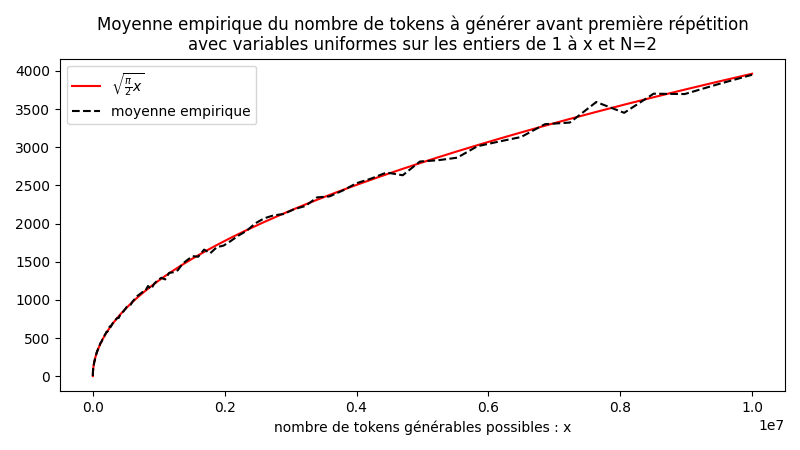
\includegraphics[scale=0.3]{images/Comparaison temps d'attente de première répétition variables uniformes N=2 et borne asymptotique.png}
    \end{center}
\end{frame}

\begin{frame}{Génération de texte "greedy" : résultats expérimentaux} % 
    \begin{center}
        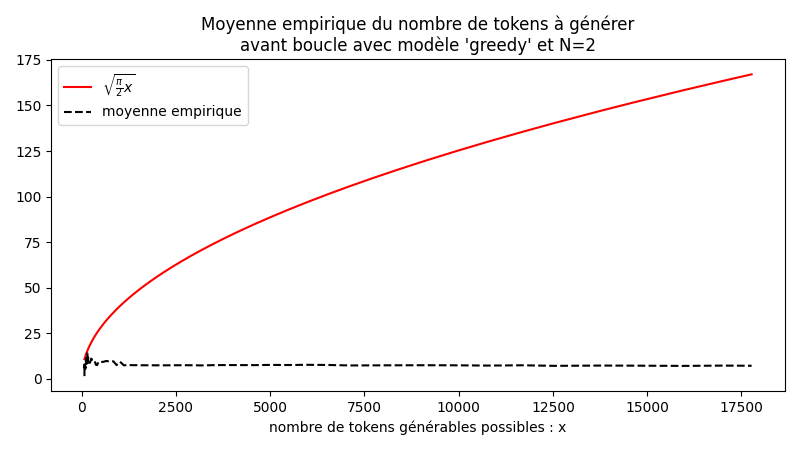
\includegraphics[scale=0.3]{images/Comparaison temps d'attente de boucle avec modèle greedy N=2 et borne asymptotique.png}
    \end{center}
    \begin{center}
        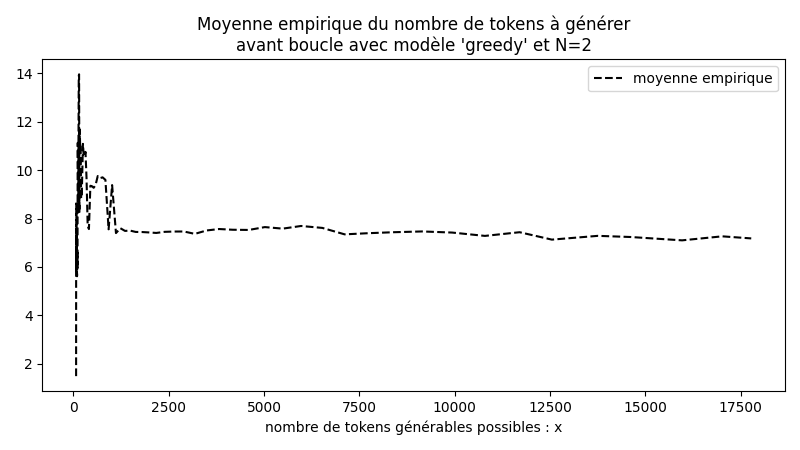
\includegraphics[scale=0.3]{images/Temps d'attente de boucle avec modèle greedy N=2.png}
    \end{center}
\end{frame}


% --- Génération de texte stochastique (aléatoire) ---
\begin{frame}[c]
    \centering
    \Huge \textcolor{MyOrange}{Génération de texte stochastique (aléatoire)} % 
\end{frame}

\begin{frame}{Génération de texte stochastique : quelques exemples} % 
    \renewcommand{\arraystretch}{2}

\begin{center}

    \begin{tabular}{|m{4cm}|m{5cm}|}

     Boucle & Pas boucle \\
    \hline

    %=================================================
    % 2 mots + boucle
    %=================================================

    \begin{center}
        \begin{tikzpicture}[
            >=Stealth,
            state/.style={
            circle,
            fill,
            inner sep=1.5pt
            }, 
            scale=1
        ]

        \node[state] (0) at (-1.4,1.4) {};
        \node[state] (1) at (0,0) {};
        
        \roundloop[135:0.5]{0}{$p$}
        \roundloop[-45:0.5]{1}{$1$}
        
        \draw[->] (0) -- node[above right] {$1-p$} (1);

        \node[above left] at (-1.4,1.4) {{\color{blue}\small 0}};
        \node[below right] at (0,0) {{\color{blue}\small 1}};

        \end{tikzpicture}
    \end{center}


    &

    %=================================================
    % 2 mots sans boucle
    %=================================================
    
    \begin{center}
        \begin{tikzpicture}[
            >=Stealth,
            state/.style={
            circle,
            fill,
            inner sep=1.5pt
            }, 
            scale=1
        ]

        \node[state] (0) at (-1.4,1.4) {};
        \node[state] (1) at (0,0) {};
        
        \roundloop[135:0.5]{0}{$p_0$}
        \roundloop[-45:0.5]{1}{$p_1$}
        
        \draw[->,bend left=20] (0) to node[above right] {$1-p_0$} (1);
        \draw[->,bend left=20] (1) to node[below left] {$1-p_1$} (0);

        \node[above left] at (-1.4,1.4) {{\color{blue}\small 0}};
        \node[below right] at (0,0) {{\color{blue}\small 1}};

        \end{tikzpicture}
    \end{center}


    \end{tabular}

    \end{center}

\end{frame}

\begin{frame}{Génération de texte stochastique : existence d'une boucle} % 
    On note l'évènement "boucle" :
    $${\scriptstyle B:=\{ \exists n_0 \in \N^*, \hspace{0.1cm} \exists l \in \N^*, \hspace{0.1cm} \exists (t_0, \cdots, t_{l-1}) \in V^l, \hspace{0.1cm} \forall Q \in \N,\hspace{0.2cm} X_{n_0 + ql + r} = t_r \hspace{0.2cm} 0 \leq r < l, \hspace{0.1cm} 0 \leq q \leq Q \} }$$
    $\space$ \\

    \pause
    \begin{tcolorbox}[
    colback=red!5,
    colframe=red!75!black,
    title=Proposition
    ]
    $\mathbb{P}_{start}(B)>0$ si, et seulement si, il existe $l \in\N^*$, il existe $C:=(t_0, \cdots, t_{l-1}) \in V^l$ tel que $p(t_i, t_{i+1}) = 1 $ pour $i \in \{0, \cdots, l-1\}$ avec $t_l := t_0$ ET $\mathbb{P}_{start}(\text{C est atteint})>0$.
    \end{tcolorbox}
    où $p(t_i, t_{i+1}) := \probacond{X_1=t_{i+1}}{X_0=t_i}$ pour tout $(t_i, t_{i+1}) \in V^2$.
\end{frame}

\begin{frame}{Génération de texte stochastique : existence d'une boucle} % 
    \begin{center}
        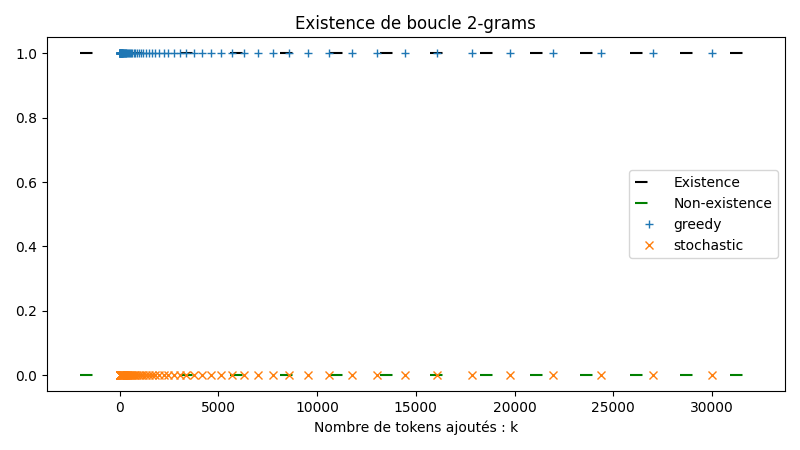
\includegraphics[scale=0.6]{images/Existence de boucle N=2.png}
    \end{center}
\end{frame}

% --- Généralisation aux chaînes de Markov d'ordre supérieur à 1 ---
\begin{frame}[c]
    \centering
    \Huge \textcolor{MyOrange}{Généralisation aux N-grams, $N > 2$} % 
\end{frame}

\begin{frame}{Chaînes de Markov d'ordre $(N-1) > 1$} % 
    Si $(X_n)_{n \in \N^*}$ chaîne de Markov d'ordre $(N-1)$ sur $V$ i.e. \\
    $\forall n \geq N-1,$
    \begin{align*}
        &{\color{white}= } \probacond{X_{n+1}=x_{n+1}}{X_1 = x_1, X_2 = x_2, ..., X_{n}=x_{n}} \\
        &= \probacond{X_{n+1}=x_{n+1}}{X_{n -(N-1) +1} = x_{n -(N-1) +1}, ..., X_{n}=x_{n}}
    \end{align*}
    \pause
    On pose
    $$ Y_{n} = \left( \begin{array}{c}
                X_{n-(N-1)+1}
                \vdots \\
                X_{n-i+1} \\
                \vdots \\
                X_{n} \\
                \end{array} \right) $$
    \pause
    $(Y_n)_{n \geq (N-1)}$ chaîne de Markov d'ordre 1 sur $V^{N-1}$. \\
\end{frame}

\begin{frame}{N-grams, $N > 2$ : résultats}
    \begin{center}
        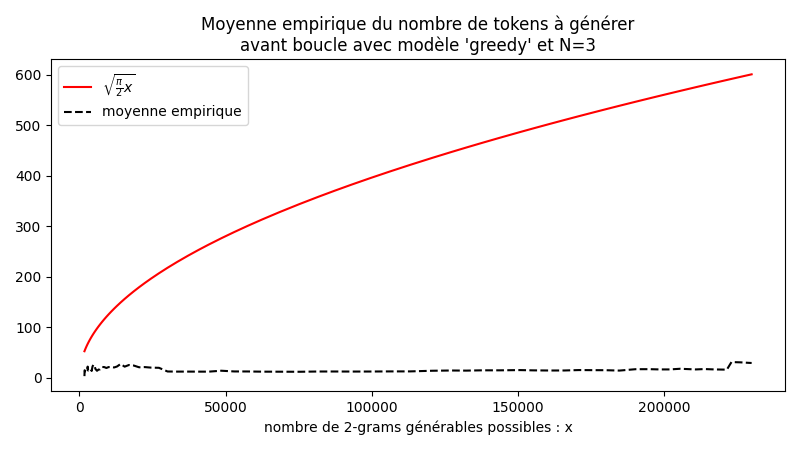
\includegraphics[scale=0.3]{images/Comparaison temps d'attente de boucle avec modèle greedy N=3 et borne asymptotique.png}
    \end{center}
    \begin{center}
        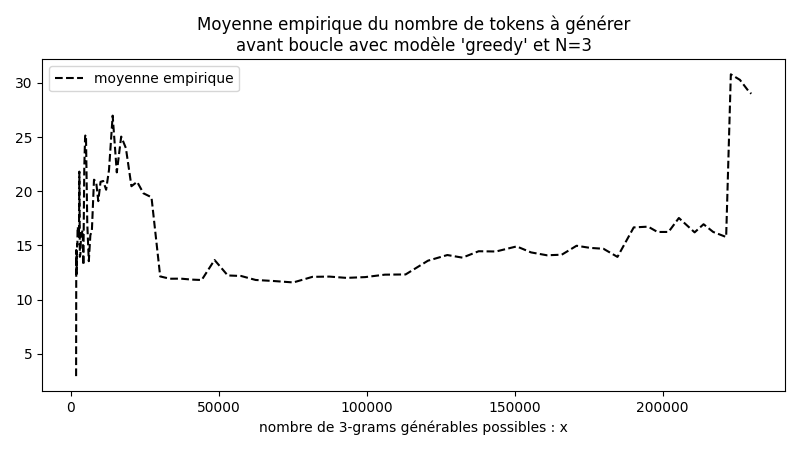
\includegraphics[scale=0.3]{images/Temps d'attente de boucle avec modèle greedy N=3.png}
    \end{center}
\end{frame}

\begin{frame}{N-grams, $N > 2$ : résultats}
    \begin{center}
        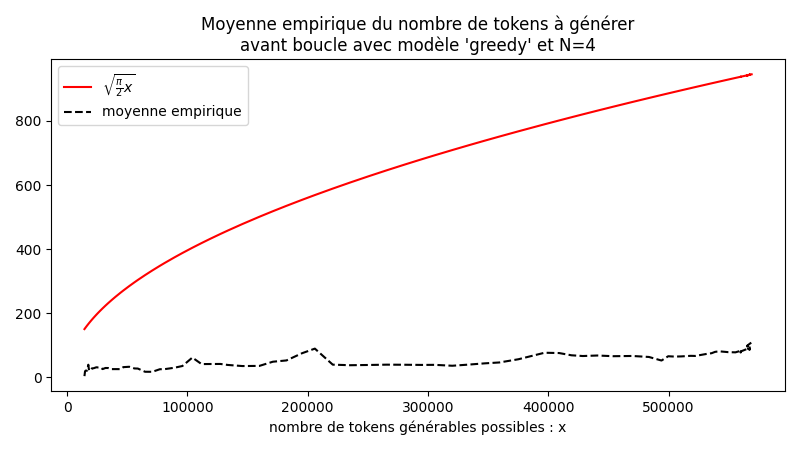
\includegraphics[scale=0.3]{images/Comparaison temps d'attente de boucle avec modèle greedy N=4 et borne asymptotique.png}
    \end{center}
    \begin{center}
        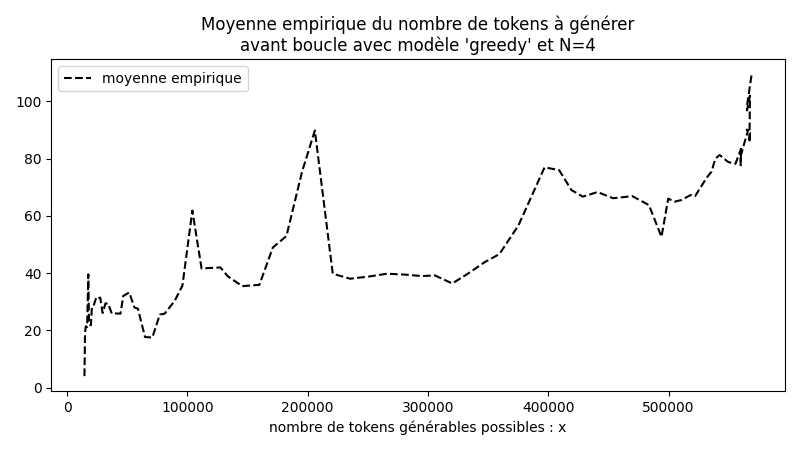
\includegraphics[scale=0.3]{images/Temps d'attente de boucle avec modèle greedy N=4.png}
    \end{center}
\end{frame}

\begin{frame}{N-grams, $N > 2$ : résultats}
    \begin{center}
        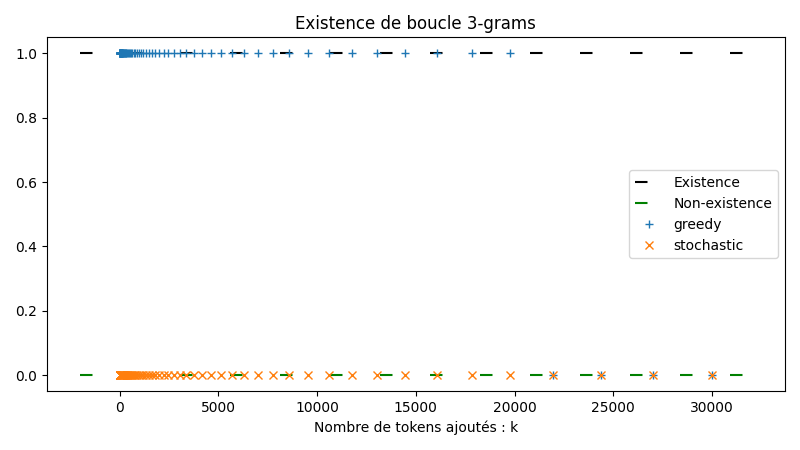
\includegraphics[scale=0.6]{images/Existence de boucle N=3.png}
    \end{center}
\end{frame}

\begin{frame}{N-grams, $N > 2$ : résultats}
    \begin{center}
        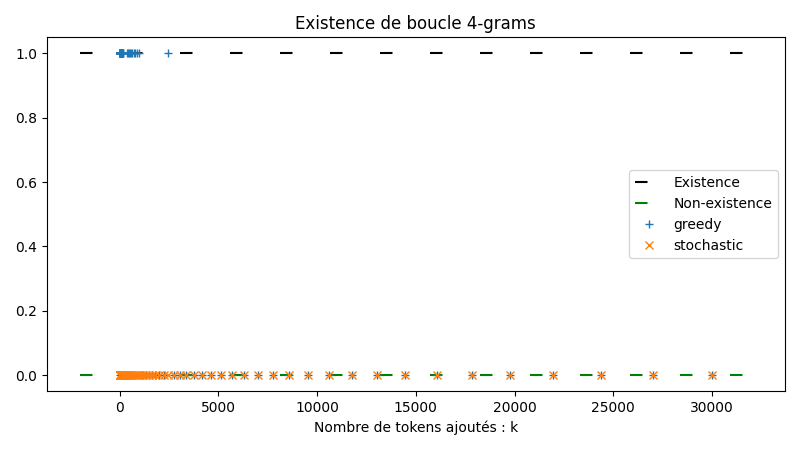
\includegraphics[scale=0.6]{images/Existence de boucle N=4.png}
    \end{center}
\end{frame}


% --- Pour aller plus loin ---
\begin{frame}[c]{Conclusion} % 
    \begin{itemize}[<+->]
        \item Existence de boucle si texte infini et modèle déterministe
        \item Caractérisation existence de boucle 
        \item Algorithme vérifiant existence de boucle 
    \end{itemize}
\end{frame}


% --- Page de fin ---
\begin{frame}[c]
    \centering
    \Huge \textcolor{MyOrange}{Merci de votre attention} % 
\end{frame}

\begin{frame}{Bibliographie}
    \textbf{[1]} D. Jurafsky, J. H. Martin, \emph{Speech and Language Processing}, $3^e$ édition, manuscrit en ligne, chapitres 2 et 3, 2026.  
    Disponible à l’adresse : \url{https://web.stanford.edu/~jurafsky/slp3} \\
    \textbf{[2]} Z. Fu, W. Lam, A. M.-C. So, B. Shi, \emph{A Theoretical Analysis of the Repetition Problem in Text Generation}, 2021, arXiv:2012.14660v4 [cs.CL]. \\
    \textbf{[3]} R. A. Horn, C. R. Johnson, \emph{Matrix Analysis}, Cambridge University Press, 2013. \\
    \textbf{[4]} J. R. Norris, \emph{Markov Chains}, Cambridge University Press, 2009. \\
    \textbf{[5]} J. Xu, \emph{Can a Higher Order Markov Chain Be Treated as a First Order Markov Chain ?}, 2025, arXiv:2512.01969 [math.PR].
\end{frame}

% --- ANNEXES ---
\begin{frame}[c]
    \centering
    \Huge \textcolor{MyOrange}{Annexes} % 
\end{frame}

% --- Les modèles N-grams ---
\begin{frame}{Les modèles N-grams : en théorie} % 
    $\forall n \in \N, \forall (m_1, ...,  m_N) \in V^N$ \\
    $$\probacond{X_{n+N} = m_N}{X_n+1=m_1, ..., X_{n+(N-1)}} = p_{m_i, ..., m_N} $$
    \\ $\space$ \\
    donc $|V|^N$ probabilités.
\end{frame}

\begin{frame}{Les modèles N-grams : en pratique}
    Applications numériques si $|V|=3\times10^4$ :
    \begin{itemize}
        \item $N=2 : \hspace{1cm} 9\times10^8$
        \item $N=3 : \hspace{1cm} 2.7\times10^{13}$
        \item $N=4 : \hspace{1cm} 8.1\times10^{17}$
    \end{itemize}

    En pratique : \\
    \begin{center}
        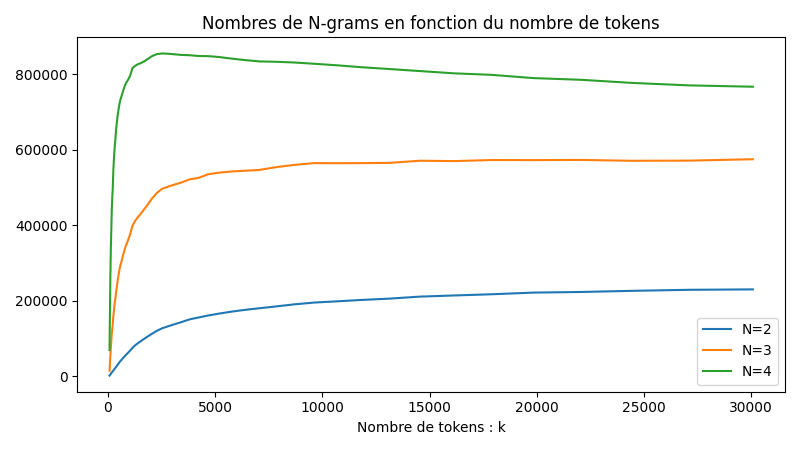
\includegraphics[scale=0.4]{images/Nombres de N-grams.png}
    \end{center}
\end{frame}

\begin{frame}{Les modèles N-grams : structure de données} % 
    Structure creuse : \\
    \hspace*{0.5cm} dictionnaire (clé = contexte) \\ %*ici les tuples (car liste pas hashable) des ids des tokens
    Besoins : \\
    \begin{itemize}
        \item Calcul de probabilités (perplexity)
        \item Génération de messages
    \end{itemize}
\end{frame}

\begin{frame}{Les modèles N-grams : simuler une variable aléatoire}
    Soit $U$ une variable aléatoire uniforme sur $[0,1]$ définie sur $(\Omega, \mathcal{F}, \mathbb{P})$.\\
    {\color{white}Soit} $p_1, ..., p_n$ des nombres de $[0,1]$ dont la somme est 1. \\
    Alors, 
    $$ X := \sum_{k=1}^{n} k \times 1_{p_1 + ... + p_{k-1} \leq U < p_1 + ... + p_{k-1} + p_k} $$
    est une variable aléatoire sur $(\Omega, \mathcal{F}, \mathbb{P})$ telle que : 
    $$ \forall k \in \{1, ..., n\}, P(X=k) = p_k $$
\end{frame}

\begin{frame}{Les modèles N-grams : structure de données} % 
    Structure creuse : dictionnaire (clé = contexte) \\ %*ici les tuples (car liste pas hashable) des ids des tokens
    Besoins : \\
    \begin{itemize}
        \item Calcul de probabilités (perplexity) \\
        \hspace{0.5cm} Dictionnaire : {token suivant : probabilité / compteur} 
        \item Génération de messages \\
        \hspace{0.5cm} {\small Liste cumulée des probabilités / compteurs et liste correspondante des tokens}
        \item Praticité \\
        \hspace{0.5cm} Compteur plutôt que probabilité \\ %add-k smoothing
        \hspace{0.5cm} Tout contexte de taille $\leq N$ \\ % interpolation
        \hspace{0.5cm} Listes rangées, puis cumulées. % greedy / top-k
    \end{itemize}
\end{frame}

\begin{frame}{L'algorithme BPE : implémentation} 
    Quelle(s) structure(s) pour le "vocabulaire" ? \\
    $\hspace*{0.5cm}$ Objectif : découper du texte en "tokens" : \\ 
    \begin{center}
        vocabulaire = \{AB, BC\} $\hspace*{1cm}$ texte à découper : "ABC"
    \end{center} 
    \begin{center}
        AB C $\hspace*{1cm}$ OU $\hspace*{1cm}$ A BC ? 
    \end{center}
    $\space$ \\
    Nécessité d'ordre sur les fusions : ordre utilisé dans l'apprentissage. \\
    $$\{(\text{token}_1, \text{token}_2) : \text{ ordre de fusion}\}$$
    %\pause 
    %$$\{(\text{id token}_1, \text{id token}_2) : \text{ id token fusionné}\}$$ \pause $$\text{ liste id vers token }; \hspace*{0.5cm} \text{ dictionnaire token vers id }$$
    % L'objectif est de tokenizer derrière, on veut garder l'ordre de fusion : identifiant de token (peut aussi permettre un gain mémoire). Mais du coup il faut garder la bijection id <-> token 
\end{frame}


\begin{frame}{L'algorithme BPE : implémentation dans les détails}
    \begin{itemize}
        \item Après fusion : mettre à jour compteur de paires et corpus \\% Garder l'indice des mots du corpus dans lesquels se retrouve chaque paire (voire la position à l'intérieur du mot)
        $\hspace*{0.5cm}$ Localiser les mots où les paires apparaissent.
        \item Récupérer le maximum du compteur de paires plusieurs fois \\
        $\hspace*{0.5cm}$ Utilisation d'un tas-max. De 35.1sec à 20.9sec : -40\% 
        \item Garder la position exacte des paires \\ % nécessite une structure particulière de liste chainée pour que ça soit efficace comparé à juste réécrire le mot à chaque fois
        Fusion (a,b) dans  x \space a \space b \space y : \hspace*{0.5cm}  x \space ab \space y \\
        paires qui changent : (x,a), (a,b), (b,y), (x,ab), (ab,y) \\
        $\hspace{0.5cm}$ Mot en liste chaînée. De 20.9sec à 13.3sec : -36\% 
        \item Les mots apparaissent plusieurs fois dans le corpus... \\ % garder une structure où chaque mot apparait une fois avec son nombre d'apparition dans le corpus et ses indices d'apparition
        $\hspace{0.5cm}$ Dictionnaire \{mot : liste chaînée, nombre d'occurences, position\}. De 12.9sec à 1.89sec : -85\% 
        \item Combien de tokens ? % 30000 cf Jurafsky
    \end{itemize}
\end{frame}

\begin{frame}{Génération de texte "greedy" : temps de première répétition} % 
    Simplification de notations : $V/=|V|$, $f:x\mapsto \exp \frac{-x^2}{2}$ \\ 
    Pour tout $k \in \{2, \cdots, V\}$ :
    \[
        \begin{aligned}
            \mathbb{P}_{t_1}(\tau > k) &= \frac{V-1}{V} \frac{V-2}{V} \cdots \frac{V - (k-1)}{V} \\
            &= \prod_{j=1}^{k-1} (1 - \frac{j}{V})
        \end{aligned}
    \]
    donc
    \[
        \mathbb{E}_{t_1}[\tau] = \sum_{k=0}^{V} \mathbb{P}_{t_1}(\tau > k) = 2 + \sum_{k=2}^{V} p_k
    \]
\end{frame}

\begin{frame}{Génération de texte "greedy" : temps moyen de première répétition} % 
    Or :
    \[
        \ln p_k = \sum_{j=1}^{k-1} \ln(1-\frac{j}{V}) \leq \sum_{j=1}^{k-1} -\frac{j}{V} = \frac{-k(k-1)}{2V}
    \] 
    donc 
    \[
        0 \leq p_k \leq \exp(\frac{-k(k-1)}{2V}) = \exp(-\frac{k}{2V}) f(\frac{k}{\sqrt{V}})
    \]
    donc si $k>\sqrt{V}$, \hspace{0.2cm}  $$\lim_{V \longrightarrow + \infty} p_k = 0$$, d'où :
    \[
        \mathbb{E}_{t_1}[\tau] = 2 + \underbrace{\sum_{k=2}^{A\sqrt{V}} p_k}_{S_1} + \underbrace{\sum_{k=A\sqrt{V}+1}^{V} p_k}_{S_2} \pause \sim \sqrt{\frac{\pi}{2}V} 
    \]
\end{frame}

\begin{frame}{Génération de texte "greedy" : calcul de $S_2$} % 
    \begin{align*}
        S_2 &\leq \sum_{k=A\sqrt{V}+1}^{V} \exp(\frac{-k(k-1)}{2V}) = \sum_{k=A\sqrt{V}+1}^{V} \exp(-\frac{k}{2V}) f(\frac{k}{\sqrt{V}}) \\ 
        &\leq \sum_{k=A\sqrt{V}+1}^{V} f(\frac{k}{\sqrt{V}}) \\
        &\leq \int_{A\sqrt{V}}^{V+1} f(\frac{x}{\sqrt{V}}) dx \\ %comparaison somme intégrale  
        &\leq \sqrt{V} \int_{A}^{\sqrt{V} + 1/\sqrt{V}} f(y) dy \leq \sqrt{V} \int_{A}^{+ \infty} f(y) dy \\ %changement de variable
    \end{align*}
    Or $\int_{A}^{+ \infty} f(y) dy \sim \frac{f(A)}{A}$, on pose $A:=V^{\alpha}$ et : $S_2 = O(V^{\frac{1}{2} - \alpha} f(V^{\alpha}))  $
\end{frame}

\begin{frame}{Génération de texte "greedy" : calcul de $S_1 $} % 
    Si $k \leq A\sqrt{V} = V^{\frac{1}{2} + \alpha}$ et $j\leq k-1$ \\
    $\frac{j}{V} \leq V^{\frac{1}{2} - \alpha}$ donc si $\alpha < \frac{1}{2}$, $\lim_{V \longrightarrow + \infty} \frac{j}{V} = 0$ \\
    \begin{align*}
        \ln p_k &= \sum_{j=1}^{k-1} \ln(1 - j/V) \\
        & = \sum_{j=1}^{k-1} - \frac{j}{V} + O(\frac{j^2}{V^2}) \\
        & = - \frac{k^2}{2V} + O(\frac{k^2}{V^2}) = - \frac{k^2}{2V} + O(V^{3\alpha - \frac{1}{2}}) \\
        p_k &= \exp(\frac{k^2}{2V}) \exp(O(V^{3\alpha - \frac{1}{2}})) \\
        &= f(\frac{k}{\sqrt{V}}) (1 + O(V^{3\alpha - \frac{1}{2}})) \text{  si } \alpha < \frac{1}{6} % si alpha < 1/6 pour que le O soit un o(1)
    \end{align*}
\end{frame}

\begin{frame}{Génération de texte "greedy" : calcul de $S_1 $} % 
    \begin{align*}
        S_1 &= \sum_{k=2}^{A\sqrt{V}} p_k \\
            &=\sum_{k=2}^{V^{\frac{1}{2} + \alpha}} f(\frac{k}{\sqrt{V}}) (1 + O(V^{3\alpha - \frac{1}{2}})) \\
            &= (1 + o(1)) \sum_{k=2}^{V^{\frac{1}{2} + \alpha}} f(\frac{k}{\sqrt{V}}) \sim \sum_{k=2}^{V^{\frac{1}{2} + \alpha}} f(\frac{k}{\sqrt{V}}) =: S_V
    \end{align*}
    Somme de Riemann de pas $\delta_V := 1/\sqrt{V}$ ? 
    $$\frac{S_V}{\sqrt{V}} = \sum_{2 \delta_V < k\delta_V \leq V^{\alpha}} \delta_V f(k\delta_V)$$
\end{frame}

\begin{frame}{Génération de texte "greedy" : calcul de $S_1 $} % 
    Soit $\epsilon > 0$ et $B>0$. 
    $$ \sum_{B < k\delta_V \leq V^{\alpha}} \delta_V f(k\delta_V) \leq \int_{B}^{+ \infty} f(x) dx \leq \epsilon \text{    pour B assez grand.} $$
    $$ \lim_{N \longrightarrow +\infty} \sum_{0 < k\delta_V \leq B} \delta_V f(k\delta_V) = \int_{0}^{B} f(x)dx $$ \\
    \text{ donc l'écart entre les deux est inférieur à } $\epsilon$ \text{ pour V assez grand. Ainsi,} \\
    $$ \sum_{0 < k\delta \leq 2\delta_V}  \delta_V f(k\delta_V) \leq \int_{0}^{3\delta_V} f(x) dx \leq \epsilon \text{    pour V assez grand.} $$
    $$|\frac{S_V}{\sqrt{V}} - \int_{0}^{+ \infty} f(x)dx| \leq 4 \epsilon $$ 
    $$\text{Finalement,   } S_1 \sim S_V \sim \sqrt{V} \int_{0}^{+ \infty} f(x)dx = \sqrt{\frac{\pi}{2}V}$$
\end{frame}

\begin{frame}{Génération de texte "greedy" : temps moyen de première répétition} % 
    \[
        \begin{aligned}
            \mathbb{E}_{t_1}[\tau] &= 2 + \underbrace{\sum_{k=2}^{A\sqrt{V}} p_k}_{S_1} + \underbrace{\sum_{k=A\sqrt{V}+1}^{V} p_k}_{S_2} \\
            &= 2 + \sqrt{\frac{\pi}{2}V} + o(1) + O(V^{\frac{1}{2} - \alpha} \exp(-\frac{V^{2\alpha}}{2})) \\
            & = \sqrt{\frac{\pi}{2}V} + o(\sqrt{V})
        \end{aligned}
    \]
    Finalement, 
    $$ \mathbb{E}_{t_1}[\tau] \sim \sqrt{\frac{\pi}{2}V} $$
\end{frame}

\begin{frame}{Génération de texte stochastique (aléatoire) : existence d'une boucle} % 
    On suppose l'existence de $C$. \\
    Si $C$ est atteint, disons en $n_0$, alors (quitte à réindexer les $x_i$) :
    $$\forall Q \in \N,\hspace{0.2cm} X_{n_0 + ql + r} = t_r \hspace{0.2cm} 0 \leq r < l, \hspace{0.1cm} 0 \leq q \leq Q$$
    donc $\{\text{C est atteint}\} \subset B$ \\
    Or $\mathbb{P}_{start}(\text{C est atteint})>0$ par hypothèse.\\
    Donc $\mathbb{P}_{start}(B)>0$.
\end{frame}

\begin{frame}{Génération de texte stochastique : existence d'une boucle} % 
    Si $\mathbb{P}_{start}(B)>0$.
    $$ B:= \bigcup_{n_0 = 0}^{+ \infty} \bigcup_{l = 1}^{+ \infty} \bigcup_{(t_0, \cdots, t_{l-1}) \in V^l} \bigcap_{Q=0}^{+\infty} \underbrace{\{X_{n_0 + ql + r} = t_r \hspace{0.2cm} 0 \leq r < l, \hspace{0.1cm} 0 \leq q \leq Q \}}_{A_Q}$$
    Soit $n_0$, $l$, $(t_0, \cdots, t_{l-1})$ tels que $\mathbb{P}_{start}(\bigcap_{Q=0}^{+\infty} A_Q) > 0$. \\ $\space$ \\
    $\bullet$ Supposons qu'il existe $s \in \{0, \cdots, l-1\}$ tel que $p(t_{s}, t_{s+1}) < 1 $ 
    \[
        \begin{aligned}
            \mathbb{P}_{start}(A_Q) &= \mathbb{P}_{start}(X = t_0) \prod_{r=1}^{l-1} p(t_r, t_{r+1}) \prod_{q=1}^{Q} \prod_{r=0}^{l-1} p(t_r, t_{r+1}) \\
            \pause &\leq 1 \prod_{q=1}^{Q} p(t_{s}, t_{s+1}) = p(t_{s}, t_{s+1})^Q
        \end{aligned}
    \]
    donc $\mathbb{P}_{start}(\bigcap_{Q=0}^{+\infty} A_Q) = \lim_{Q \longrightarrow +\infty} \mathbb{P}_{start}(A_Q) = 0$ ,  contradiction.
\end{frame}

\begin{frame}{Généralisation aux chaînes de Markov d'ordre $(N-1) > 1$} % 
    Soit $(t_{2}, \cdots, t_{(N-1)+1})$ et $(j_{1}, \cdots, j_{(N-1)})$ dans $S^{N-1}$. \\
    Si $t_k = j_k$ pour $2 \leq k \leq (N-1)$ alors :
    \begin{align*}
        &\probacond{Y_{n+1} = (t_{2}, \cdots, t_{(N-1)+1}) }{Y_{1} = y_{1}, \cdots,Y_{n} = (j_{1}, \cdots, j_{(N-1)})} \\
        &= \probacond{X_{n-(N-1)+2} = t_{2}, \cdots , X_{n+1} = t_{(N-1)+1} }{X_{1} = x_{1}, \cdots,X_{n} = j_{(N-1)}} \\
        &= \probacond{X_{n+1} = t_{(N-1)+1}}{X_{n-(N-1)+1} = j_{1}, \cdots,X_{n} = j_{(N-1)}} = p_{j_{1} \cdots j_{(N-1)} t_m} \\
        &{\scriptstyle = \probacond{X_{n-(N-1)+2} = t_{2}, \cdots , X_{n+1} = t_{(N-1)+1}}{X_{n-(N-1)+1} = j_{1}, \cdots,X_{n} = j_{(N-1)}}} \\
        &= \probacond{Y_{n+1} = (t_{2}, \cdots, t_{(N-1)+1}) }{Y_{n} = (j_{1}, \cdots, j_{(N-1)})} 
    \end{align*}
    Sinon le résultat reste (et la probabilité est nulle). \\
    $(Y_n)_{n \geq (N-1) }$ chaîne de Markov d'ordre 1 sur $S^{N-1}$. \\
\end{frame}

\end{document}
